\documentclass[11pt]{article}

\usepackage[a4paper,margin=1in]{geometry}
\usepackage{amsmath,amssymb}
\usepackage{booktabs}
\usepackage{microtype}
\usepackage{xcolor}
\usepackage{tikz}
\usepackage[hidelinks]{hyperref}

\newcommand{\pending}[1]{\textcolor{red}{\textbf{[#1]}}}
\newcommand{\hex}[1]{\texttt{#1}}

\title{The six-round differential optimum of ARADI is 82:\\
a machine-checked lower bound}

\author{Nobuo Otoi\\
\small \texttt{ba-cybersecurity.com}, Tokyo, Japan\\
\small ORCID: 0009-0001-1445-3612}

\date{November 2026}

\begin{document}
\maketitle

\begin{abstract}
The automated study of the NSA block cipher ARADI by Bellini et al.\ (\emph{CLAASPing ARADI}, INDOCRYPT~2024) reports in its Table~4 that the best single-key differential trail over six rounds has weight~84, printed in bold to denote optimality. Using the authors' own CLAASP model of ARADI we show that this value is not optimal: a single-key differential trail of weight~82 exists over six rounds, and no trail of weight~81 or less exists. The upper bound is a weight-82 trail of CLAASP's S-box model, confirmed by re-fixing it in the model and by the designers' round-function formula; CLAASP's own search returns weight-82 trails directly, and Monte-Carlo estimation agrees. The lower bound is obtained by a hybrid CNF (CLAASP's own component clauses together with a bidirectional sequential-counter encoding of the weight and Matsui-style window constraints), split by cube-and-conquer into 945 subproblems, every one of which is UNSAT; all 945 UNSAT results, together with the twenty one-to-five-round Matsui bounds they rely on, carry a DRAT certificate verified by \texttt{drat-trim}. The six-round optimum of 82 is therefore the first machine-checked optimal differential weight reported for round-reduced ARADI. The same weight-82 trail is also optimal under CLAASP's bit-sliced (AND-gate-count) model, whose six-round optimum we likewise show to be 82, so 84 is not optimal in either weight definition. The seven- and eight-round upper bounds of 106 and 122 in Table~4 are reproduced and thereby confirmed. We report the result as a single corrected table cell supported by a reproducible certificate, not as a break of the cipher. The result is a small example of machine-checked cybersecurity analysis: its central claim rests on a DRAT certificate that an independent checker re-verifies, not on a solver's unsupported word.
\end{abstract}

\section{Introduction}

ARADI is a 128-bit block cipher with a 256-bit key, designed by Greene, Motley and Weeks of the NSA for low-latency memory encryption~\cite{aradi}. Its differential behaviour over a reduced number of rounds was analysed automatically by Bellini et al.~\cite{claasping} with the CLAASP framework~\cite{claasp}; their Table~4 lists, for one to ten rounds, the weight of the best single-key differential trail found, with the entries claimed optimal printed in bold.

\paragraph{Contribution.} We determine the exact optimal single-key differential weight of ARADI over six rounds, show it to be \textbf{82} rather than the 84 printed as optimal in Table~4 of~\cite{claasping}, and give the first machine-checked (DRAT) certificate of a round-reduced differential lower bound for this cipher. The nearest prior work is \cite{claasping} itself: it reports the six-round weight, but as a solver output without a verified lower bound, and the reported value is not optimal under its own definition. The weight-82 trail and the weight-$\le 81$ lower-bound instance both use \cite{claasping}'s own clause generator for trail validity, so the discrepancy cannot be attributed to a difference of definition; the tool is sound and the reported value is simply not optimal.

\paragraph{Scope.} This is a single corrected entry with a reproducible proof, not an attack. We do not claim any improvement in the cryptanalytic security margin of full ARADI, and we are careful below to separate what is certified from what is only strongly supported.

\section{Preliminaries}

\paragraph{ARADI.} We use the designers' specification~\cite{aradi}. The 128-bit state is four 32-bit words $w\,\|\,x\,\|\,y\,\|\,z$. Each round applies a 4-bit S-box (realised as a four-gate Toffoli circuit) in bit-sliced form across the 32 columns, followed by a linear layer and a round-key addition. We verified that CLAASP reproduces the designers' test vector \hex{0x3f09abf400e3bd7403260defb7c53912}; our own S-box and linear layer agree with the designers' rotation amounts, constants and S-box, and with CLAASP on all two-round differential trails of weight 8, the two-round optimum (\S\ref{sec:method}).

\paragraph{Two CLAASP models of the weight.} CLAASP offers two cipher objects for ARADI, and they induce two differential-weight definitions:
\begin{itemize}
  \item \emph{S-box model} (\texttt{AradiBlockCipherSBox} with \texttt{SatXorDifferentialModel}). Each active S-box contributes $4-\log_2(\mathrm{DDT})\in\{0,2,3\}$ and the linear layer and key addition are deterministic. This is the model of~\cite{claasping}, \S6.1 and Listing~1.6, and the one that reproduces Table~4; it is our principal model.
  \item \emph{Bit-sliced model} (\texttt{AradiBlockCipher}). Here the weight is the number of active AND (Toffoli) gates. We use it only as an independent cross-check of the main result (\S\ref{sec:modelind}); \cite{claasping} itself notes that the bit-sliced version yields less accurate differential probabilities, consistent with Table~4 being computed in the S-box model.
\end{itemize}
In both models the optimum over $r$ rounds is the smallest weight $w$ such that a trail of weight $w$ exists and no trail of weight $w-1$ exists, in the single-key setting (key difference fixed to zero, plaintext difference non-zero), exactly as in Table~4.

\paragraph{Matsui bounds.} For a window of $r$ consecutive rounds beginning at round index $s \bmod 4$ we write $B_s[r]$ for a lower bound on the trail weight of that window. We established, for every starting index, the exact one-to-five-round optima
\[
B[1\mathinner{..}5] = 2,\,8,\,14,\,32,\,50,
\]
each proved by an UNSAT instance with a DRAT certificate (\S\ref{sec:verify})---four of them over CLAASP's own CNF, the remaining sixteen over an independent S-box model of ours that we validate against CLAASP by the full two-round enumeration of \S\ref{sec:method} (identical sets of all 39{,}168 weight-8 two-round trails), by the matching one-to-five-round optima, and by the designers' linear layer. These agree with the one-to-five-round entries of Table~4.

\section{Method}
\label{sec:method}

\paragraph{Hybrid CNF for the lower bound.} To prove that no six-round trail of weight $\le 81$ exists we build a CNF with three parts:
\begin{enumerate}
  \item the component clauses that CLAASP itself emits for the six-round S-box model (\texttt{build\_xor\_differential\_trail\_model} with no weight counter), so that the set of satisfying assignments is exactly CLAASP's set of valid trails;
  \item a bidirectional sequential counter over the per-S-box Hamming-weight variables, asserting that the total weight is at most 81;
  \item Matsui-style window clauses: for each sub-window $[s,e]$ the prefix and suffix weights are bounded below by the corresponding $B$ values above, which prunes the search without removing any trail of weight $\le 81$.
\end{enumerate}
Because part~1 is taken verbatim from CLAASP, a counting or encoding bug could at worst make the instance spuriously UNSAT. We rule that out: the \emph{same} hybrid CNF with the bound raised to 82 is satisfiable and returns a weight-82 trail, so the UNSAT at 81 is genuine and not an artefact of over-constraint. We also checked the component clauses directly, by full enumeration of the S-box relation and by matching every weight-8 two-round trail against CLAASP's model.

\paragraph{Cube-and-conquer.} The six-round, weight-$\le 81$ instance is partitioned by the first- and second-round weights. With $w_0$ the first-round weight and $w_{01}$ the weight of the first two rounds, the Matsui bounds confine the feasible region to
\[
w_0 \in [2,\,31], \qquad w_{01}\in[w_0+2,\,49],
\]
which yields \textbf{945} cubes (Figure~\ref{fig:cubes}). Each cube is a unit-clause file appended to the base CNF and solved independently by \texttt{kissat} in \texttt{--unsat} mode with proof logging. All 945 are UNSAT; their union is the whole instance, so the six-round optimum is at least 82.

\begin{figure}[t]
\centering
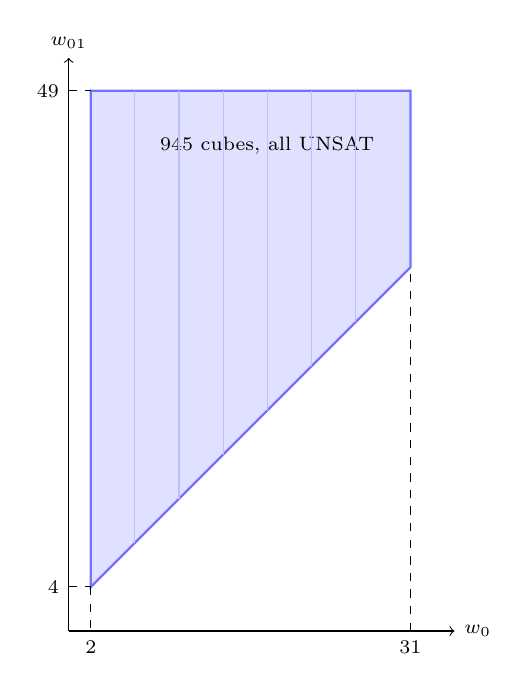
\begin{tikzpicture}[scale=0.14]
  % axes
  \draw[->] (0,0) -- (35,0) node[right] {\scriptsize $w_0$};
  \draw[->] (0,0) -- (0,52) node[above] {\scriptsize $w_{01}$};
  % feasible region: w0 in [2,31], w01 in [w0+2, 49]
  \fill[blue!12] (2,4) -- (31,33) -- (31,49) -- (2,49) -- cycle;
  \draw[blue!55,thick] (2,4) -- (31,33) -- (31,49) -- (2,49) -- cycle;
  % diagonal lower edge label
  \node at (18,44) {\scriptsize 945 cubes, all UNSAT};
  \draw[dashed] (2,4) -- (2,0) node[below] {\scriptsize 2};
  \draw[dashed] (31,0) node[below] {\scriptsize 31} -- (31,33);
  \draw[dashed] (0,49) node[left] {\scriptsize 49} -- (2,49);
  \draw[dashed] (0,4) node[left] {\scriptsize 4} -- (2,4);
  % example grid lines
  \foreach \x in {6,10,14,18,22,26} {\draw[blue!25] (\x,\x+2) -- (\x,49);}
\end{tikzpicture}
\caption{Cube-and-conquer partition of the six-round weight-$\le 81$ instance by $(w_0,w_{01})$. The Matsui bounds $B[1\mathinner{..}5]=2,8,14,32,50$ confine the feasible pairs to the shaded region; each integer pair in it is one cube. Vertical lines indicate the per-$w_0$ slices.}
\label{fig:cubes}
\end{figure}

\paragraph{Upper bound.} The weight-82 trail of Table~\ref{tab:perround} is a valid trail of CLAASP's S-box model: re-fixing its seven state differences in the unconstrained CLAASP model gives total weight 82, while the same fixing at weight 81 is UNSAT, and its weight is independently recomputed by the designers' round-function formula (82). CLAASP's \texttt{SatXorDifferentialModel} also returns weight-82 trails directly (for instance at bound 83 in 23\,s and at bound 82 in 141\,s), and Monte-Carlo estimation over $2^{22}$ pairs per round on weight-82 trails agrees ($\approx 82$); the upper bound is thus confirmed by several independent routes.

\paragraph{Certificates.} Each UNSAT instance---the 945 six-round cubes and the twenty one-to-five-round Matsui bounds---is solved with \texttt{kissat} emitting a binary DRAT proof, which is independently checked by \texttt{drat-trim}~\cite{drattrim}. A run is accepted only on \texttt{drat-trim}'s \texttt{VERIFIED} verdict.

\section{Results}
\label{sec:results}

\paragraph{Six rounds: optimum 82.} In the S-box model of~\cite{claasping} the optimal single-key differential weight over six rounds is exactly 82. A weight-82 trail exists (upper bound), and no trail of weight $\le 81$ exists (lower bound, certified). Table~4 of~\cite{claasping} prints 84 in bold for six rounds; under its own definition this is not optimal. The per-round S-box weights of the certified weight-82 trail are shown in Table~\ref{tab:perround}; its plaintext difference is \hex{0x000000002854044a0000000000000000}.

\begin{table}[t]
\centering
\begin{tabular}{lcccccc r}
\toprule
round & 1 & 2 & 3 & 4 & 5 & 6 & total\\
\midrule
S-box weight & 18 & 6 & 18 & 16 & 8 & 16 & 82\\
\bottomrule
\end{tabular}
\caption{Per-round S-box weights of the certified six-round weight-82 trail. The same round profile holds for the bit-sliced (AND-gate) model (\S\ref{sec:modelind}).}
\label{tab:perround}
\end{table}

\paragraph{Lower bound, certified.} All 945 cubes of the weight-$\le 81$ instance are UNSAT, with DRAT certificates verified by \texttt{drat-trim}; their trail-validity clauses are CLAASP's own. The Matsui bounds the window pruning relies on are likewise DRAT-certified (four over CLAASP's own CNF, sixteen over our CLAASP-validated S-box model, as noted above). The six-round lower bound of 82 is therefore machine-checked, with that single modelling dependence made explicit. Resource figures are in \S\ref{sec:verify}.

\paragraph{Model independence.}
\label{sec:modelind}
We repeated the check in CLAASP's bit-sliced model, where the weight counts active AND gates. There too the six-round optimum is 82. The upper bound is the same state trail: fixing its differences in CLAASP's real bit-sliced CNF gives SAT at 82 and UNSAT at 81, with the per-round AND-gate profile $[18,6,18,16,8,16]$ of Table~\ref{tab:perround}. For the lower bound we used a compressed model (a ``T-model'' that counts, per S-box column, the minimum number of active AND gates realising the column's input/output difference) which we prove equivalent to CLAASP's bit-sliced model by a lemma, validated against the real bit-sliced CNF on the one-to-four-round optima (the four-round case by an 800-cube DRAT campaign), on a partial five-round check (305 of 1{,}568 cubes, all UNSAT), and on three known trails; in that model weight 81 is UNSAT, certified by the same cube-and-conquer method (945/945 cubes DRAT-verified, together with an unconstrained \texttt{kissat} UNSAT). The bit-sliced six-round optimum is therefore also 82. The S-box lower bound uses CLAASP's own clauses for trail validity, drawing only its Matsui window bounds from the CLAASP-validated model above; this bit-sliced lower bound rests more heavily on re-modelling, through the hand-proved equivalence lemma, so we treat it as the weaker of the two. Either way, 84 is not optimal in either weight definition.

\paragraph{Seven and eight rounds.} Trails of weight 106 (seven rounds) and 122 (eight rounds) exist in the S-box model, matching the values in Table~4. These are upper bounds found by SAT; we did not certify them as optimal, and we report them as a confirmation of Table~4, not a correction. A bounded search below these weights was inconclusive within our time budget and is not claimed either way.

\section{Verification and reproducibility}
\label{sec:verify}

The 945 six-round UNSAT certificates were produced and checked in a single campaign: 945/945 \texttt{VERIFIED}, 0 failures; total 22.47 CPU-hours (11.88\,h solving and proof generation, 10.59\,h \texttt{drat-trim} verification) and 1\,h\,54\,m of wall time; the hardest cube took 286\,s to solve and 261\,s to verify with a 307\,MB proof. The proofs total 36.3\,GB and were deleted after verification; the SHA-256 of each proof and the full \texttt{drat-trim} logs are retained. The twenty Matsui-bound instances (five-round at each of the four starting indices, and the one-to-four-round bounds) were certified the same way. The bit-sliced lower bound of \S\ref{sec:modelind} was certified by a separate campaign of 945/945 UNSAT cubes (all DRAT-verified) in the equivalent T-model, taking 66.8 CPU-hours (31.3\,h solving, 35.5\,h verification) and 3\,h\,12\,m of wall time.

The artefacts for independent reproduction are: the CLAASP-model driver; the hybrid-CNF generator; the cube generator and runner; the fixed-trail certificate checker; the weight-82 trails; and the per-cube summary tables with solve times, verdicts and proof hashes. The exact CLAASP commit (\texttt{f2239d6}, version~v3.2.0) is pinned, solved with \texttt{kissat}~4.0.4 and checked with \texttt{drat-trim}; CLAASP's own clause generator was run under a minimal SageMath shim, whose clause output we validated by the full S-box enumeration and two-round trail match of \S\ref{sec:method}, and a full SageMath install at the same commit is expected to emit identical clauses. These artefacts, together with this manuscript, are deposited in a public archive at DOI~\texttt{10.5281/zenodo.24025026} (concept DOI, resolving to the latest version); we do not reproduce customer or third-party data.

The remaining open items are stated plainly: the bit-sliced lower bound rests on an equivalence lemma proved by hand (\S\ref{sec:modelind}), not on a DRAT proof over CLAASP's own bit-sliced clauses, and we flag it as such; the printed INDOCRYPT proceedings version of Table~4 (DOI \texttt{10.1007/978-3-031-80311-6\_5}) was not inspected directly, and we cite the ePrint version~\cite{claasping}; and we found no prior published correction of this entry. One natural explanation for the printed 84---that it was computed in the bit-sliced model---is refuted by \S\ref{sec:modelind}: the bit-sliced six-round optimum is also 82, so 84 is not optimal there either. We have no confirmed explanation for the printed value, only that it is not optimal under either definition.

\section{Honest use of AI}

The research question (``is the six-round entry of Table~4 optimal?''), the claims made here, and the check of every number against the primary result files were decided and carried out by the author, Nobuo Otoi. The search for trails and the SAT/UNSAT computations were executed by an AI coding assistant (Claude Code) under the author's direction. The lower bound does not rest on the assistant's or the solver's word: each UNSAT result is an independent DRAT certificate checked by \texttt{drat-trim}, and the upper bound is a trail re-verified by the designers' formula and by Monte-Carlo estimation. The assistant's own reading of the work is not treated as a review or as independent evidence.

\begin{thebibliography}{9}

\bibitem{aradi}
P.~Greene, M.~Motley, and B.~Weeks.
\newblock ARADI and LLAMA: Low-Latency Cryptography for Memory Encryption.
\newblock IACR Cryptology ePrint Archive, Report 2024/1240, 2024.
\newblock \url{https://eprint.iacr.org/2024/1240}.

\bibitem{claasping}
E.~Bellini, M.~Formenti, D.~G\'erault, J.~Grados, A.~Hambitzer, Y.~J.~Huang,
P.~Huynh, M.~Rachidi, R.~Rohit, and S.~K.~Tiwari.
\newblock CLAASPing ARADI: Automated Analysis of the ARADI Block Cipher.
\newblock In \emph{INDOCRYPT 2024}, pp.~90--113.
\newblock IACR Cryptology ePrint Archive, Report 2024/1324, 2024.
\newblock \url{https://eprint.iacr.org/2024/1324}.

\bibitem{claasp}
E.~Bellini et al.
\newblock CLAASP: a Cryptographic Library for the Automated Analysis of
Symmetric Primitives.
\newblock Software framework, Crypto-TII.
\newblock \url{https://github.com/Crypto-TII/claasp}.

\bibitem{drattrim}
N.~Wetzler, M.~J.~H.~Heule, and W.~A.~Hunt~Jr.
\newblock DRAT-trim: Efficient Checking and Trimming Using Expressive Clausal
Proofs.
\newblock In \emph{SAT 2014}, pp.~422--429, 2014.
\newblock \url{https://github.com/marijnheule/drat-trim}.

\bibitem{kissat}
A.~Biere et al.
\newblock Kissat SAT Solver.
\newblock \url{https://github.com/arminbiere/kissat}.

\end{thebibliography}

\end{document}
